\documentclass[pdf, usepdftitle=false]{beamer}
%Summary of beamer themes https://www.hartwork.org/beamer-theme-matrix/
\usetheme{Frankfurt}
\usecolortheme{whale}
%Blue on slides is 51,51,178
%This is quite a dark blue so I have created my own colour
%For shades, multiply each component by 1/4, 1/2, 3/4, etc. of its previous value, depending on how dark the color should be.
%For tints, calculate (255 - previous value), multiply that by 1/4, 1/2, 3/4, etc. and add that to the previous value.
%51+204*0.25 = 102
%178+77*0.25= 197
\definecolor{lightblue}{RGB}{102,102,197}
\setbeamercolor{section in head/foot}{fg=white, bg=lightblue}
\setbeamercolor{frametitle}{fg=white, bg=lightblue}
\setbeamercolor{title}{fg=white, bg=lightblue}


\title{Title of my talk}
\author{\textbf{Author name} \\ [\baselineskip]
    Position\\
    Affiliation
    }

\date{Date}

%\setbeamertemplate{footline}[frame number] %frame number at bottom
\setbeamertemplate{footline}{} %Nothing in the footer
\setbeamertemplate{frametitle}[default][center, shadow=false] %Remove shadow from frametitle
\beamertemplatenavigationsymbolsempty %Suppress navigation bar
\setbeamertemplate{itemize items}[circle] %Itemized items use a circle
\setbeamertemplate{title page}[default][colsep=-4bp,rounded=true] %removes shadow from title page

\usepackage[T1]{fontenc} % Remove warnings about substituting fonts Font shape `OML/lmss/m/n' undefined(Font) using `OML/cmm/m/it' instead(Font) for symbol `textgreater' 
\usepackage{lmodern} %Remove warnings about missing fonts: Font shape `OT1/cmss/m/n' in size <4> not available(Font) size <5> substituted
\usepackage{textcomp} %Remove warnings about subsituting fonts Font shape `OMS/lmss/m/n' undefined(Font) using `OMS/cmsy/m/n' instead(Font) for symbol `textbullet'

\usepackage{xcolor} %Change colour of text

\newcommand{\ToDo}[1]{\textcolor{red}{\textsf{\textbf{#1}}}} %Creates a new command that hightlights text in red

\begin{document}

%\maketitle
\begin{frame}[plain]
\titlepage
\begin{columns}
\begin{column}{0.33\textwidth}
\begin{figure}[b]

\includegraphics[width=\textwidth]{BWHlogo}
\end{figure}
\end{column}
\begin{column}{0.33\textwidth}
\begin{figure}[b]

\includegraphics[width=\textwidth]{HMS}
\end{figure}
\end{column}
\begin{column}{0.33\textwidth}
\begin{figure}[b]

\includegraphics[width=\textwidth]{broad}
\end{figure}
\end{column}
\end{columns}
\end{frame}

\section{Introduction}
\subsection{}

\begin{frame}
\frametitle{Introduction} 
\begin{columns}
\begin{column}{1.1\textwidth}
\begin{figure}[H]
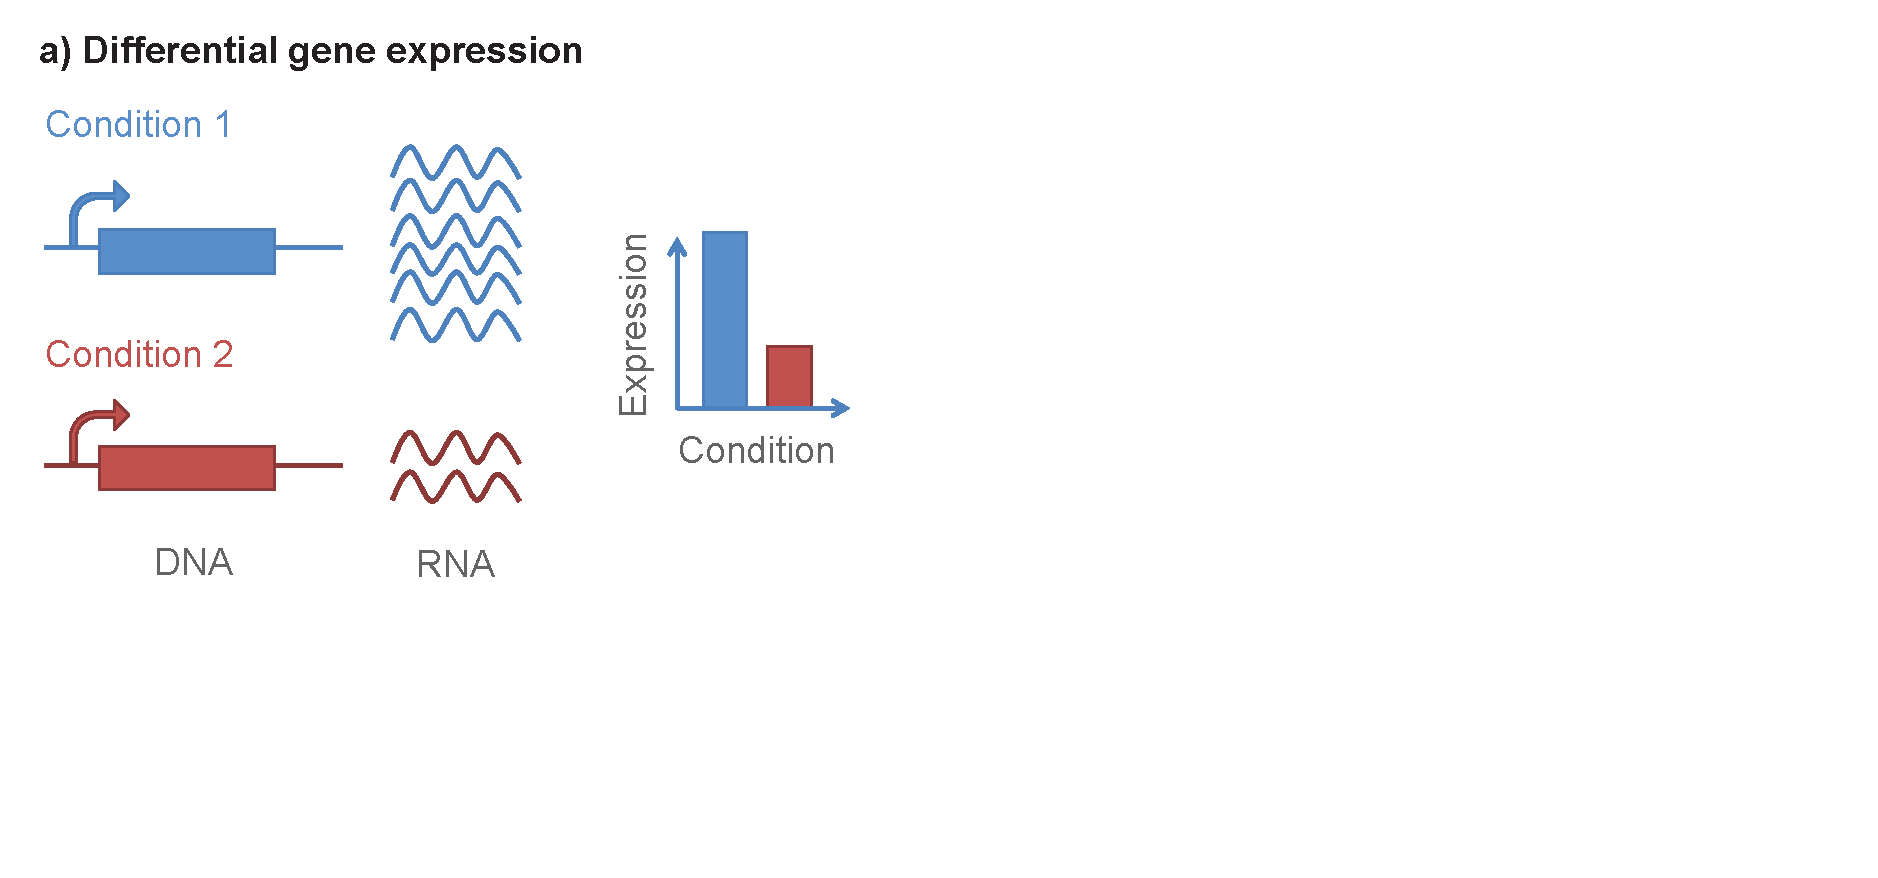
\includegraphics[width=\textwidth]{Diffex.pdf}
\end{figure}
\end{column}
\end{columns}
\end{frame}


\section{Methods}
\subsection{}
\begin{frame}
\frametitle{Methods}

\textbf{Here are the methods}\\
\vspace{0.5cm}
RNA-seq
\begin{itemize}
\item Item 1
\item Item 2
\end{itemize}

\vspace{0.5cm}
Genotyping
\begin{itemize}
\item Item 1
\end{itemize}
\end{frame}

\section{Results}
\subsection{}
\begin{frame}
\frametitle{Results 1}

\end{frame}

\begin{frame}
\frametitle{Results 2}

\end{frame}

\section{Acknowledgements}
\subsection{}
\begin{frame}
\frametitle{Acknowledgements} 

\vspace{1.5cm}


\centering
\textbf{Raychaudhuri lab}\\
\vspace{1.5cm}

\begin{columns}
\begin{column}{0.33\textwidth}
\begin{figure}[b]

\includegraphics[width=\textwidth]{BWHlogo}
\end{figure}
\end{column}
\begin{column}{0.33\textwidth}
\begin{figure}[b]

\includegraphics[width=\textwidth]{HMS}
\end{figure}
\end{column}
\begin{column}{0.33\textwidth}
\begin{figure}[b]

\includegraphics[width=\textwidth]{broad}
\end{figure}
\end{column}
\end{columns}
\end{frame}


\section[]{Extra slides} %This stops the slides being seen on the progression bar at the top


\begin{frame}
\frametitle{Extra slide}
Extra content
\end{frame}


\end{document}